%%%%%%%%%%%%%%%%%%%%%%%%%%%%%%%%%%%%%%%%%
% Wenneker Assignment
% LaTeX Template
% Version 2.0 (12/1/2019)
%
% This template originates from:
% http://www.LaTeXTemplates.com
%
% Authors:
% Vel (vel@LaTeXTemplates.com)
% Frits Wenneker
%
% License:
% CC BY-NC-SA 3.0 (http://creativecommons.org/licenses/by-nc-sa/3.0/)
% 
%%%%%%%%%%%%%%%%%%%%%%%%%%%%%%%%%%%%%%%%%

%----------------------------------------------------------------------------------------
%	PACKAGES AND OTHER DOCUMENT CONFIGURATIONS
%----------------------------------------------------------------------------------------

\documentclass[11pt]{scrartcl} % Font size

%%%%%%%%%%%%%%%%%%%%%%%%%%%%%%%%%%%%%%%%%
% Wenneker Assignment
% Structure Specification File
% Version 2.0 (12/1/2019)
%
% This template originates from:
% http://www.LaTeXTemplates.com
%
% Authors:
% Vel (vel@LaTeXTemplates.com)
% Frits Wenneker
%
% License:
% CC BY-NC-SA 3.0 (http://creativecommons.org/licenses/by-nc-sa/3.0/)
% 
%%%%%%%%%%%%%%%%%%%%%%%%%%%%%%%%%%%%%%%%%

%----------------------------------------------------------------------------------------
%	PACKAGES AND OTHER DOCUMENT CONFIGURATIONS
%----------------------------------------------------------------------------------------
\usepackage{listings}
\usepackage{xcolor}

\definecolor{codegreen}{rgb}{0,0.6,0}
\definecolor{codegray}{rgb}{0.5,0.5,0.5}
\definecolor{codepurple}{rgb}{0.58,0,0.82}
\definecolor{backcolour}{rgb}{0.95,0.95,0.92}

\lstdefinestyle{mystyle}{
    backgroundcolor=\color{backcolour},   
    commentstyle=\color{codegreen},
    keywordstyle=\color{magenta},
    numberstyle=\tiny\color{codegray},
    stringstyle=\color{codepurple},
    basicstyle=\ttfamily\footnotesize,
    breakatwhitespace=false,         
    breaklines=true,                 
    captionpos=b,                    
    keepspaces=true,                 
    numbers=left,                    
    numbersep=5pt,                  
    showspaces=false,                
    showstringspaces=false,
    showtabs=false,                  
    tabsize=2
}

\lstset{style=mystyle}
\usepackage{amsmath, amsfonts, amsthm} % Math packages

\usepackage{listings} % Code listings, with syntax highlighting

\usepackage[english]{babel} % English language hyphenation

\usepackage{graphicx} % Required for inserting images
\graphicspath{{Figures/}{./}} % Specifies where to look for included images (trailing slash required)

\usepackage{booktabs} % Required for better horizontal rules in tables

\numberwithin{equation}{section} % Number equations within sections (i.e. 1.1, 1.2, 2.1, 2.2 instead of 1, 2, 3, 4)
\numberwithin{figure}{section} % Number figures within sections (i.e. 1.1, 1.2, 2.1, 2.2 instead of 1, 2, 3, 4)
\numberwithin{table}{section} % Number tables within sections (i.e. 1.1, 1.2, 2.1, 2.2 instead of 1, 2, 3, 4)

\setlength\parindent{0pt} % Removes all indentation from paragraphs

\usepackage{enumitem} % Required for list customisation
\setlist{noitemsep} % No spacing between list items

%----------------------------------------------------------------------------------------
%	DOCUMENT MARGINS
%----------------------------------------------------------------------------------------

\usepackage{geometry} % Required for adjusting page dimensions and margins

\geometry{
	paper=a4paper, % Paper size, change to letterpaper for US letter size
	top=2.5cm, % Top margin
	bottom=3cm, % Bottom margin
	left=3cm, % Left margin
	right=3cm, % Right margin
	headheight=0.75cm, % Header height
	footskip=1.5cm, % Space from the bottom margin to the baseline of the footer
	headsep=0.75cm, % Space from the top margin to the baseline of the header
	%showframe, % Uncomment to show how the type block is set on the page
}

%----------------------------------------------------------------------------------------
%	FONTS
%----------------------------------------------------------------------------------------

\usepackage[utf8]{inputenc} % Required for inputting international characters
\usepackage[T1]{fontenc} % Use 8-bit encoding

\usepackage{fourier} % Use the Adobe Utopia font for the document

%----------------------------------------------------------------------------------------
%	SECTION TITLES
%----------------------------------------------------------------------------------------

\usepackage{sectsty} % Allows customising section commands

\sectionfont{\vspace{6pt}\centering\normalfont\scshape} % \section{} styling
\subsectionfont{\normalfont\bfseries} % \subsection{} styling
\subsubsectionfont{\normalfont\itshape} % \subsubsection{} styling
\paragraphfont{\normalfont\scshape} % \paragraph{} styling

%----------------------------------------------------------------------------------------
%	HEADERS AND FOOTERS
%----------------------------------------------------------------------------------------

\usepackage{scrlayer-scrpage} % Required for customising headers and footers

\ohead*{} % Right header
\ihead*{} % Left header
\chead*{} % Centre header

\ofoot*{} % Right footer
\ifoot*{} % Left footer
\cfoot*{\pagemark} % Centre footer
 % Include the file specifying the document structure and custom commands

%----------------------------------------------------------------------------------------
%	TITLE SECTION
%----------------------------------------------------------------------------------------

\title{	
	\normalfont\normalsize
	\textsc{\Huge Physics-1 Lab SM203P}\\ % Your university, school and/or department name(s)
	\vspace{25pt} % Whitespace
	\rule{\linewidth}{0.5pt}\\ % Thin top horizontal rule
	\vspace{20pt} % Whitespace
	{\huge Experiment 2: Experiments with simple and double pendulums with phase portraits}\\ % The assignment title
	\vspace{12pt} % Whitespace
	\rule{\linewidth}{2pt}\\ % Thick bottom horizontal rule
	\vspace{12pt} % Whitespace
}

\author{\Huge Group-16\\
\\
\LARGE Mayank Chadha(IMT2020045)\\
\\
\LARGE Anshul Jindal(IMT2020039)\\
\\
\LARGE Rahul Jain(IMT2020117)\\
\\
\LARGE Karanjit Saha(IMT2020003)\\
\\
\LARGE Chinmay Parekh(IMT2020069)\\
\\
\LARGE Shashank Shekhar(IMT2020112)} % Your name

\date{\normalsize\today} % Today's date (\today) or a custom date

\begin{document}

\maketitle % Print the title
%----------------------------------------------------------------------------------------
%	FIGURE EXAMPLE
%----------------------------------------------------------------------------------------

\begin{figure}[h] % [h] forces the figure to be output where it is defined in the code (it suppresses floating)
	\centering
	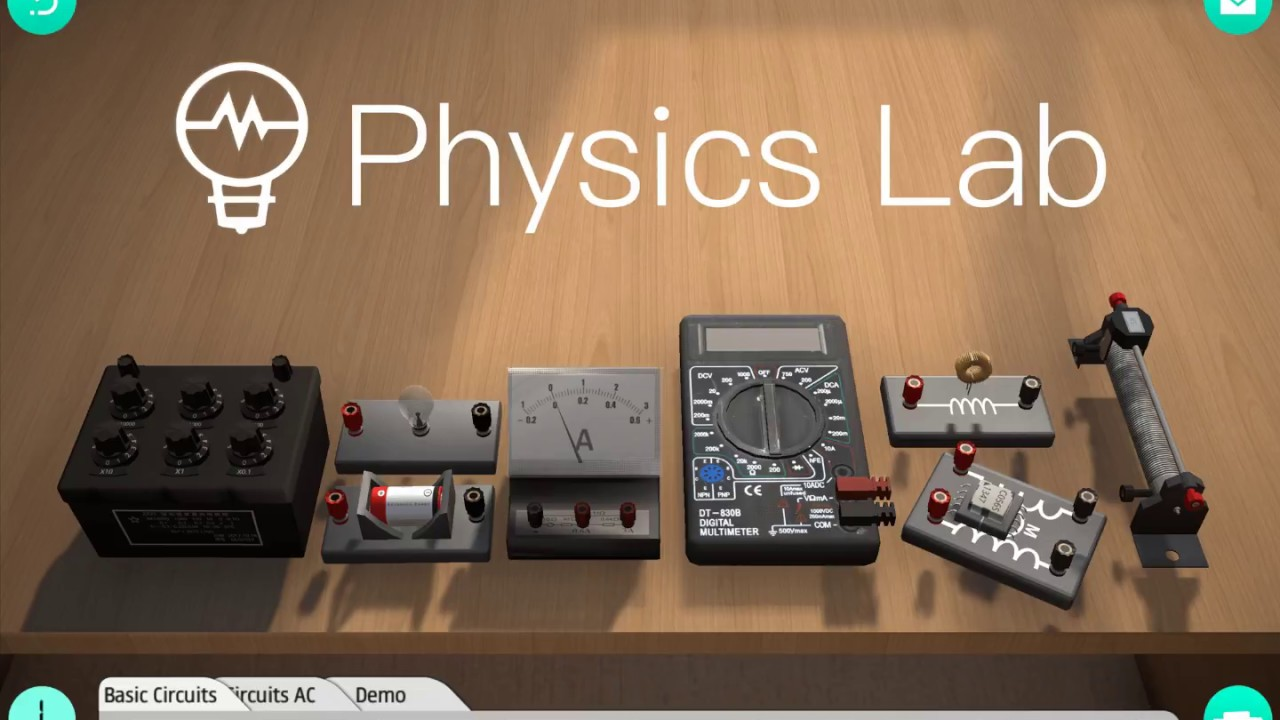
\includegraphics[width=\textwidth, height=5cm]{first.jpg} % Example image
	\caption{Physics lab.}
\end{figure}

%------------------------------------------------
\section{Aim of Experiment}
1. Find g using your phone as a simple pendulum. \par
2. Showing phase portraits and plotting time series for single and double pendulums.\par
3. Calculate the percentage dissipation of energy in the presence of drag. \par

\section{Apparatus required for the Experiment}
\begin{enumerate}
	\item A string
	\item Phyphox app
	\item Mobile phone or any solid object
	\item Simulation enviornment (https://www.myphysicslab.com/)
\end{enumerate}





%----------------------------------------------------------------------------------------
%	TEXT EXAMPLE
%----------------------------------------------------------------------------------------

%------------------------------------------------
\section{Theory}


\subsection{Acceleration Due to Gravity for Single Pendulum(g)}

We will use the Phyphox app and our mobile as a solid object tied with a string and hung like a pendulum, and the g shown shall be reported. Instead of mobile, we can also use any solid object (such as a stone ). In this case, we will note down the period of our oscillation and the length of the string. After that, to calculate g, we will use a well-known relation between the period of simple pendulum and g: \par

\begin{align} 
	\begin{split}
		T = 2\pi\sqrt{\frac{L}{g}}\\
	\end{split}					
\end{align}

Rearranging the terms, we get:
\begin{align} 
	\begin{split}
		g = \frac{4\pi^2L}{T^2}\\
	\end{split}					
\end{align}

where\\ g = acceleration due to gravity.\\ T= Time period of simple pendulum.\\ L= Length of string. \par

%------------------------------------------------

\subsection{Phase Portraits}
Phase portrait is the graph between..... $\theta$ For a simple pendulum with small amplitude(i.e. $\sin\theta \approx \theta$), phase portrait is generally an \textbf{ellipse} in an ideal case. As we increase the amplitude of the pendulum ($\theta$), we will observe the increase in length of both major and minor axis of the ellipse. \\
In the presence of viscous forces such as drag, then we observe phase portrait as concentric ellipses. In this case, we can quantify energy lost per cycle in the decrease in the area of 2 consecutive concentric ellipses (percentage decrease).

Formula for the \textbf{area(A)} of the ellipse with major axis as \textbf{a} and minor axis as \textbf{b} is:
\begin{align} 
	\begin{split}
		A = \pi ab \nonumber\\
	\end{split}					
\end{align}

\subsubsection{Liouville's Theorem}
For Non-Dissipative systems, the average phase space traversed is conserved.

%------------------------------------------------
\subsection{Time Series}
Time Series is the graph between... For non-dissipative systems, the amplitude remains constant throughout, and no energy is lost, whereas, for dissipative systems, amplitude keeps on decreasing with time, and energy also decreases along.

\subsection{Double Pendulum}
Lagrangian equation for double pendulum is as follows:

%-----------------MAYANK CHADHA WRITE ALL EQUATIONS HERE_______________________%




\section{Sources of Error}
\begin{enumerate}
	\item Air Resistance
	\item Old Tennis ball
	\item Rigged Meter Scale
	\item Inclined or Rough Surface
	\item The value of e may change with the height.
	\item Time taken during the collision will also contribute to the wrong calculation of e
	\item Phyphox mobile app uses various sensors present in a mobile phone, which may not give accurate results every time.
	\item Electric and magnetic fields may disturb the working of the sensors, due to which the results observed may not be completely accurate.
	\item Acoustic stopwatch of the Phyphox app also takes some time to stop the timer after hearing the sound of the collision.
	\item Random error.
\end{enumerate}
%----------------------------------------------------------------------------------------
%	EQUATION EXAMPLES
%----------------------------------------------------------------------------------------
\newpage

\section{Observation and Calculation}
\subsection{Mayank Chadha(IMT2020045)}

\textbf{2a}.
Phase portrait of a simple pendulum without dissipation is an ellipse.\\
Three different values of the amplitude($\theta$) taken by me is: 1.5, 1 and 0.75\\

The plot for phase portrait for all of them is shown below:

\begin{figure}[h] % [h] forces the figure to be output where it is defined in the code (it suppresses floating)
	\centering
	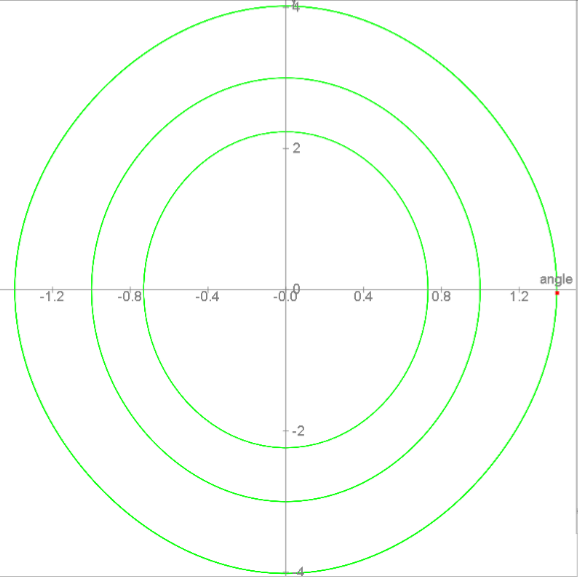
\includegraphics[width=\textwidth, height=15cm]{Figures/M 2a.png} % Example image
	\caption{Phase portrait for amplitude 1.5, 1 and 0.75.}
\end{figure}

\newpage
\textbf{2b}.
Phase Portrait of the desired experiment is:
\begin{figure}[h] % [h] forces the figure to be output where it is defined in the code (it suppresses floating)
	\centering
	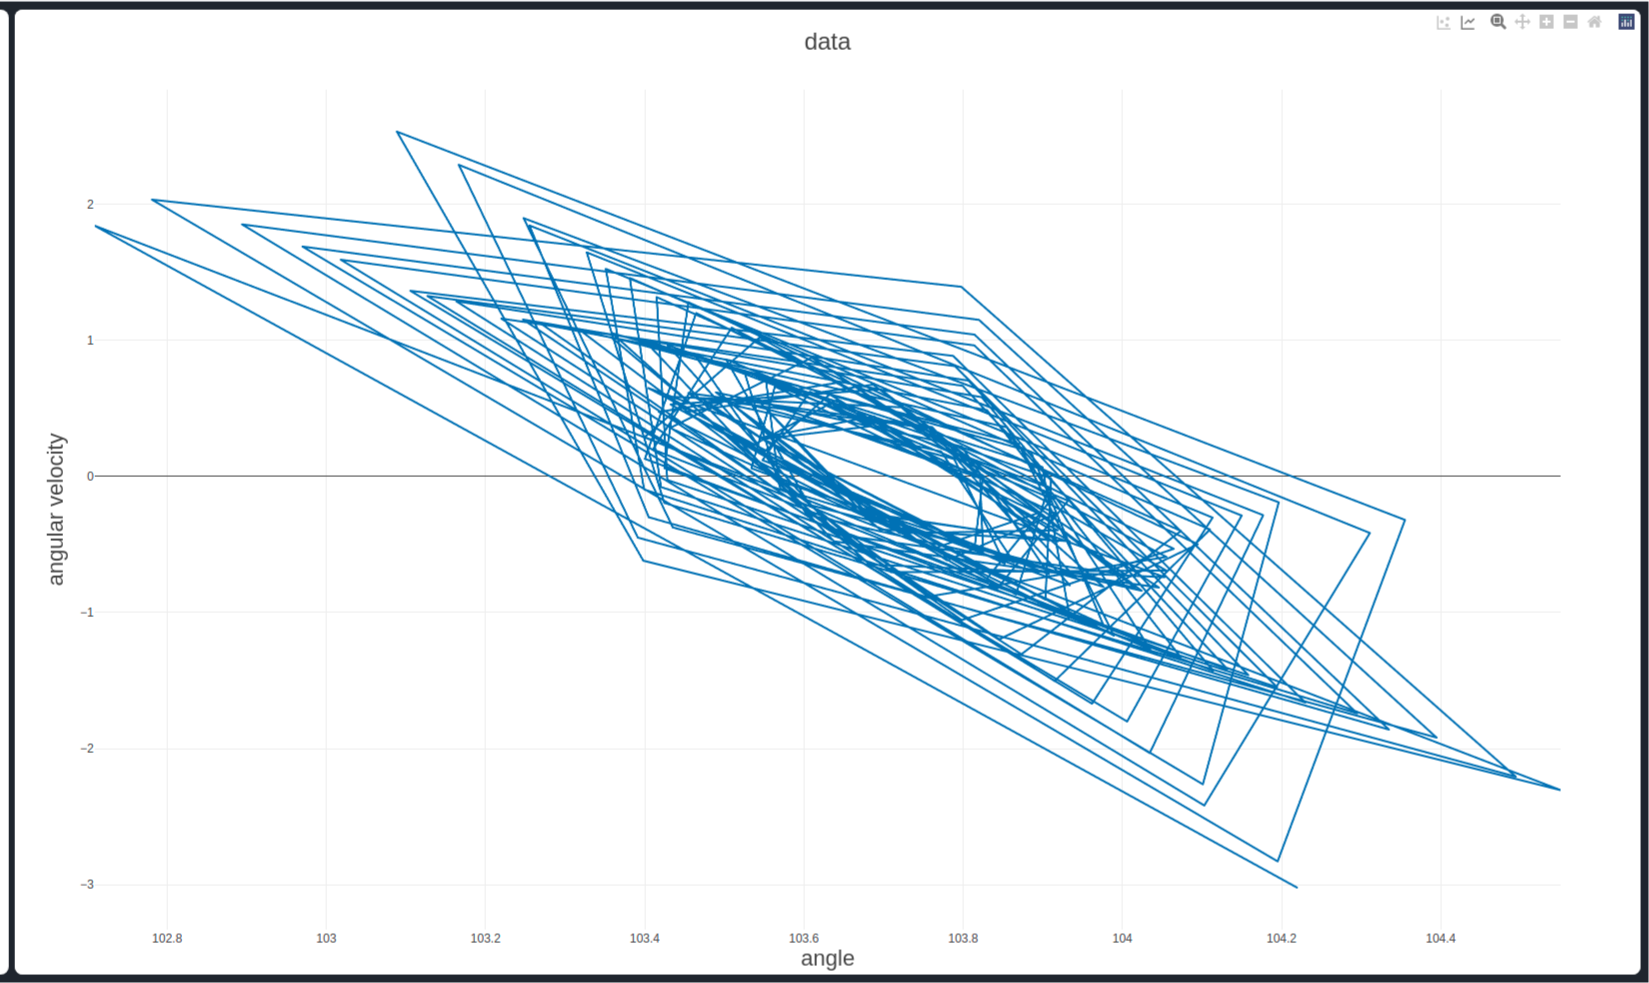
\includegraphics[width=12cm, height=8cm]{Figures/M 2b.png} % Example image
	\caption {Representative phase portrait for your smartphone-pendulum}
\end{figure}

\textbf{2c}.
Time series of the desired experiment is:
\begin{figure}[h] % [h] forces the figure to be output where it is defined in the code (it suppresses floating)
	\centering
	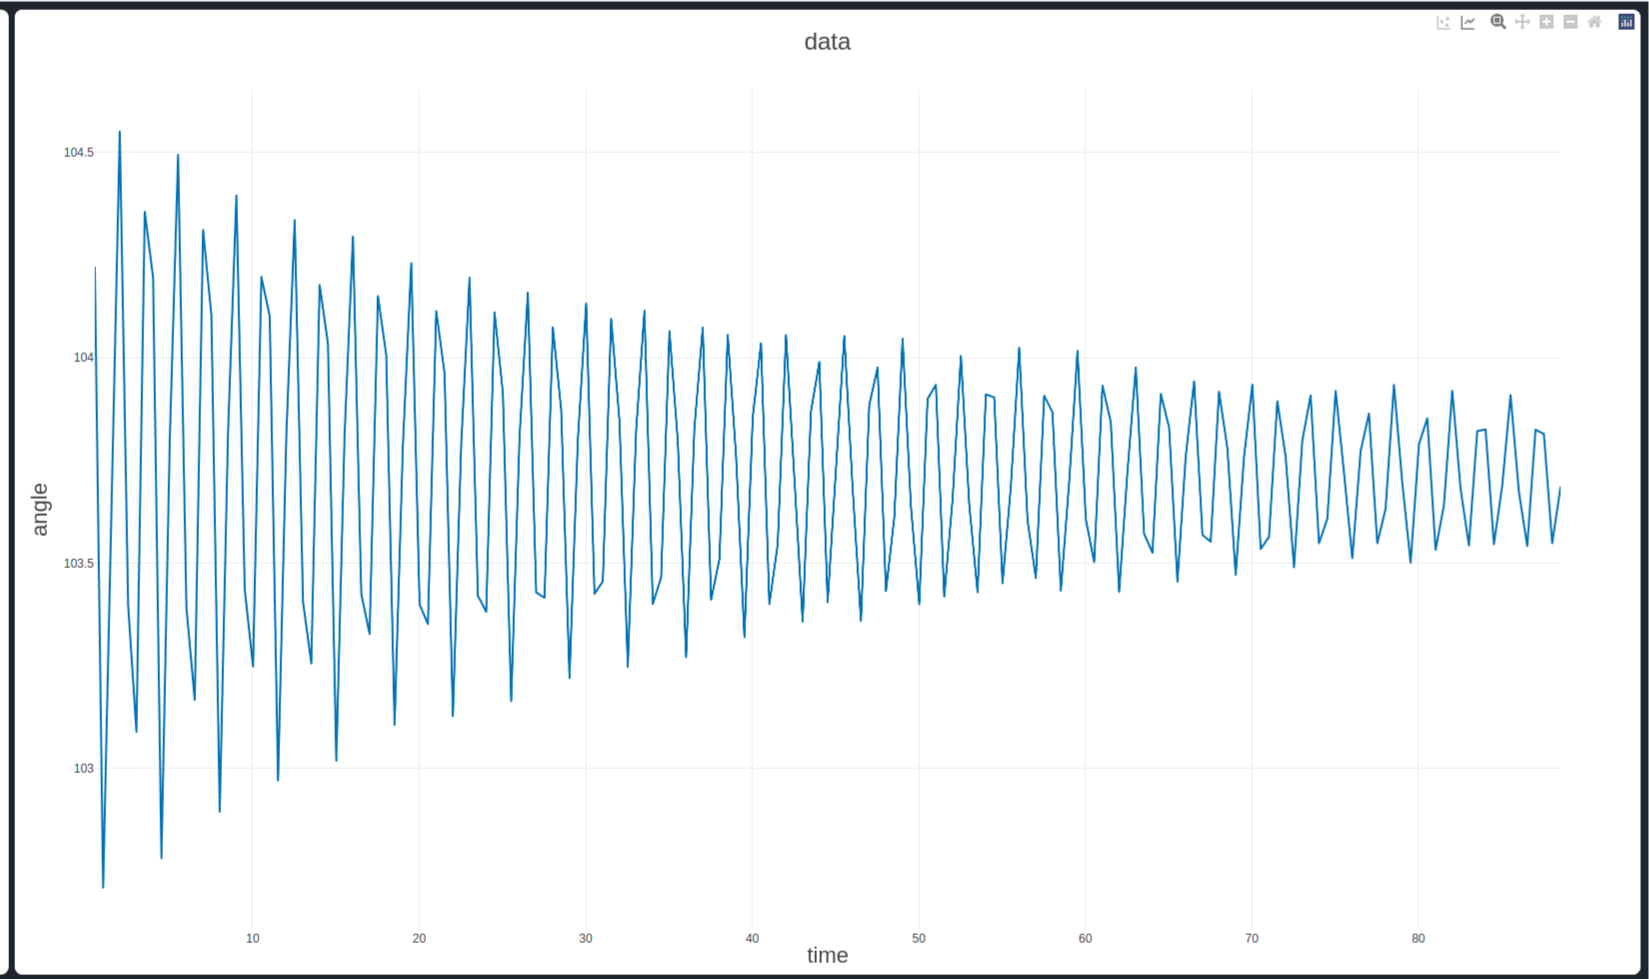
\includegraphics[width=12cm, height=8cm]{Figures/M 2c.png} % Example image
	\caption {Representative Time series for your smartphone-pendulum ($\theta$ vs t)}
\end{figure}

\newpage
\textbf{3}.
Non-zero value for the drag chosen by me = 1.870 \\
I got concentric ellipses. Phase portrait is shown below:
\begin{figure}[h] % [h] forces the figure to be output where it is defined in the code (it suppresses floating)
	\centering
	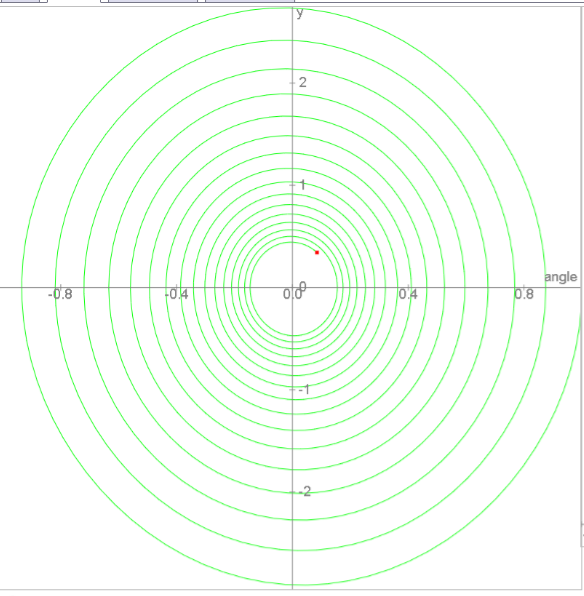
\includegraphics[width=\textwidth, height=15cm]{Figures/M3.png} % Example image
	\caption{Phase portrait for simple pendulum in presence of drag.}
\end{figure}

\textbf{$1^{st}$ Ellipse - }\\
length of major axis (a) = 2.42  units\\
length of minor axis (b) = 0.99 units\\

So area will be (A) = $\pi$ab \implies 2.42*0.99*$\pi$ \implies 2.39$\pi$ units\\
\textbf{$2^{nd}$ Ellipse - }\\
length of major axis (a) = 2.19 units\\
length of minor axis (b) = 0.89 units\\

So area will be (A) = $\pi$ab \implies 2.19*0.89*$\pi$ \implies 1.94$\pi$ units\\

\textbf{$3^{rd}$ Ellipse - }\\
length of major axis (a) = 2.09 units\\
length of minor axis (b) = 0.76 units\\

So area will be (A) = $\pi$ab \implies 2.09*0.72*$\pi$ \implies 1.52$\pi$ units\\

\textbf{Quantifying Energy Lost:}\\
Between Ellipse 1 and Ellipse 2:\\

Area of ellipse 1 (A1) = 2.39$\pi$ units\\
Area of ellipse 2 (A2) = 1.94$\pi$ units\\

Now percentage decrease in area:
\begin{equation*}
\implies (\frac{A1-A2}{A1})*100
\end{equation*}

\begin{equation*}
\implies (\frac{2.39\pi-1.94\pi}{2.39\pi})*100
\end{equation*}

\begin{equation*}
\implies 18.82 \%
\end{equation*}

Between Ellipse 2 and Ellipse 3:\\

Area of ellipse 2 (A2) = 1.94$\pi$ units\\
Area of ellipse 3 (A3) = 1.52$\pi$ units\\

Now percentage decrease in area:
\begin{equation*}
\implies (\frac{A2-A3}{A2})*100
\end{equation*}

\begin{equation*}
\implies (\frac{1.94\pi-1.52\pi}{1.94\pi})*100
\end{equation*}

\begin{equation*}
\implies 18.79 \%
\end{equation*}

\textbf{Observation:}
The percentage decrease in area is almost equal for all the consecutive concentric ellipses.\\

\textbf{4a}.
I have taken \textbf{l1} and \textbf{l2} both equal to 1.00 units such that \textbf{L}=$\frac{l2}{l1}$ = 1 units\\

The phase portraits and time series graphs are shown in next page.

The value of \textbf{M} chosen by me is $\frac{1}{2}$ units for which I took \textbf{m1} as 2.00 units and \textbf{m2} as 2.00 units.\newpage

\textbf{Phase Portrait:}\\
Below shown is the phase portrait for the double pendulum w.r.t m1:
\begin{figure}[h] % [h] forces the figure to be output where it is defined in the code (it suppresses floating)
	\centering
	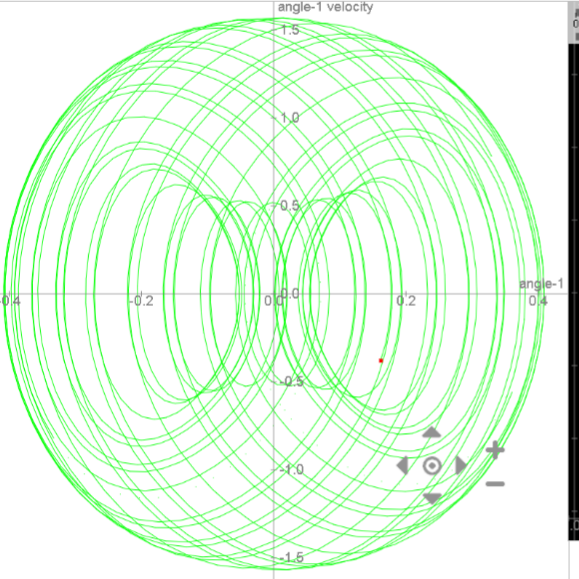
\includegraphics[width=12cm, height=8cm]{Figures/M 4b l is 1.png} % Example image
	\caption{Phase portrait for double pendulum (d$\theta_{1}$/dt vs $\theta_{1}$)}
\end{figure}
\\
Below shown is the phase portrait for the double pendulum w.r.t m2:
\begin{figure}[h] % [h] forces the figure to be output where it is defined in the code (it suppresses floating)
	\centering
	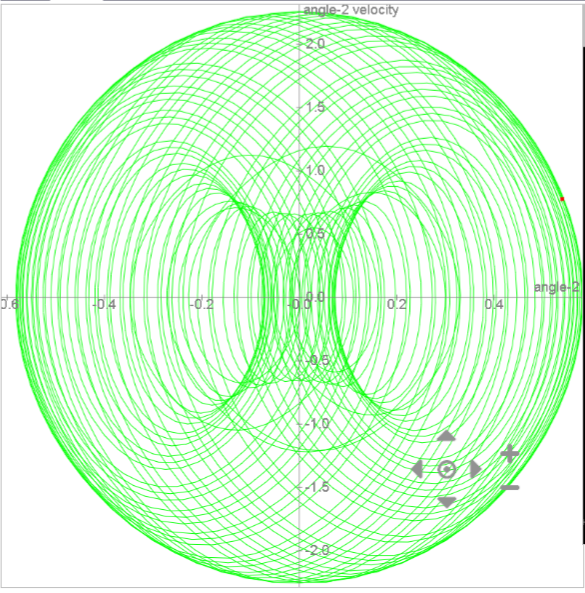
\includegraphics[width=12cm, height=8cm]{Figures/M 4b when l is 1.png} % Example image
	\caption{Phase portrait for double pendulum (d$\theta_{2}$/dt vs $\theta_{2}$)}
\end{figure}
\newpage
\textbf{Time Series:}\\
Below shown is the Time series for the double pendulum w.r.t m1:
\begin{figure}[h] % [h] forces the figure to be output where it is defined in the code (it suppresses floating)
	\centering
	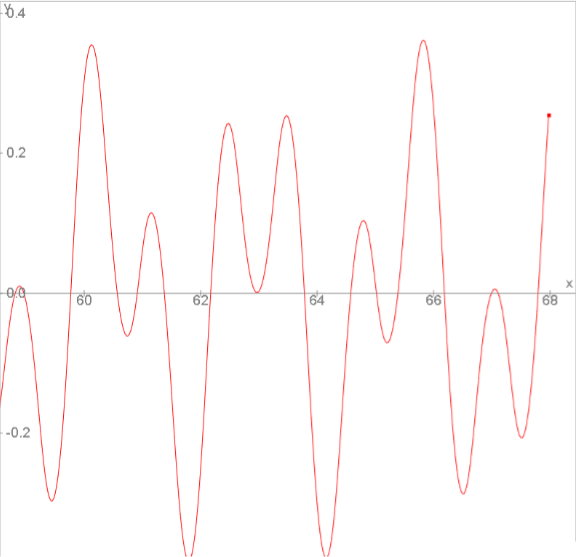
\includegraphics[width=12cm, height=8cm]{Figures/M 4a angle 1 (1).png} % Example image
	\caption{Time series for double pendulum ($\theta_{1}$ vs t)}
\end{figure}

Below shown is the Time series for the double pendulum w.r.t m2:
\begin{figure}[h] % [h] forces the figure to be output where it is defined in the code (it suppresses floating)
	\centering
	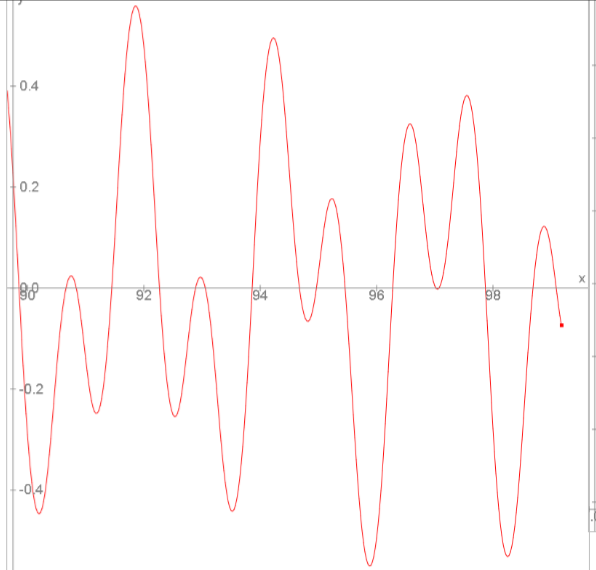
\includegraphics[width=12cm, height=8cm]{Figures/M 4a angle 2.png} % Example image
	\caption{Time series for double pendulum ($\theta_{2}$ vs t)}
\end{figure}


\newpage
\textbf{4b}.
\textbf{M} is kept constant at 0.50 units by keeping \textbf{m1} = 2.00 units and \textbf{m2} = 2.00 units as well.\\

The value of \textbf{L} chosen by me is 0.50 units by keeping \textbf{l2} = 1.000 units and \textbf{l1} = 1.000 units

\textbf{Phase Portrait:}\\
Below shown is the phase portrait for the double pendulum w.r.t m1:
\begin{figure}[h] % [h] forces the figure to be output where it is defined in the code (it suppresses floating)
	\centering
	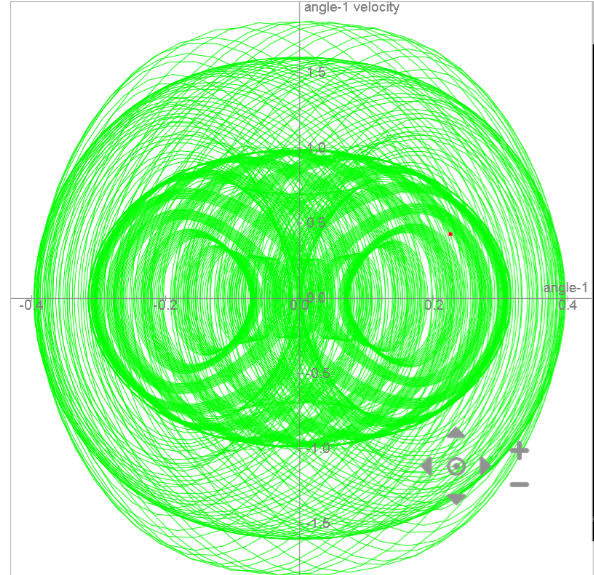
\includegraphics[width=12cm, height=8cm]{Figures/M 4b less than 1.png} % Example image
	\caption{Phase portrait for double pendulum (d$\theta_{1}$/dt vs $\theta_{1}$)}
\end{figure}
\\
Below shown is the phase portrait for the double pendulum w.r.t m2:
\begin{figure}[h] % [h] forces the figure to be output where it is defined in the code (it suppresses floating)
	\centering
	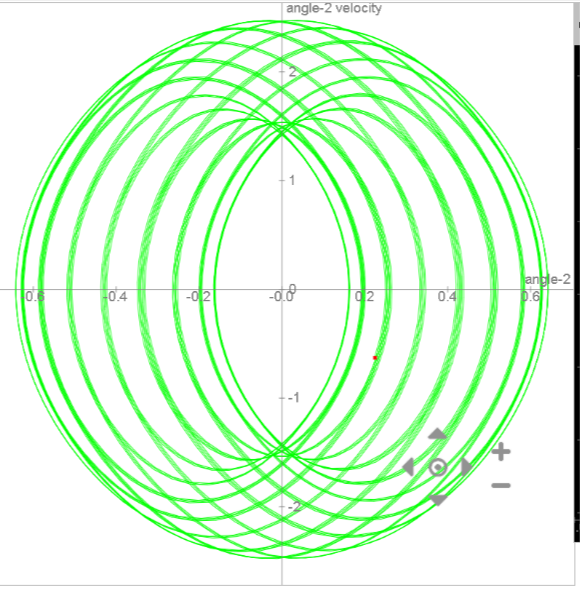
\includegraphics[width=12cm, height=8cm]{Figures/M 4b less than 1 (2).png} % Example image
	\caption{Phase portrait for double pendulum (d$\theta_{2}$/dt vs $\theta_{2}$)}
\end{figure}
\newpage
\textbf{Time Series:}\\
Below shown is the Time series for the double pendulum w.r.t m1:
\begin{figure}[h] % [h] forces the figure to be output where it is defined in the code (it suppresses floating)
	\centering
	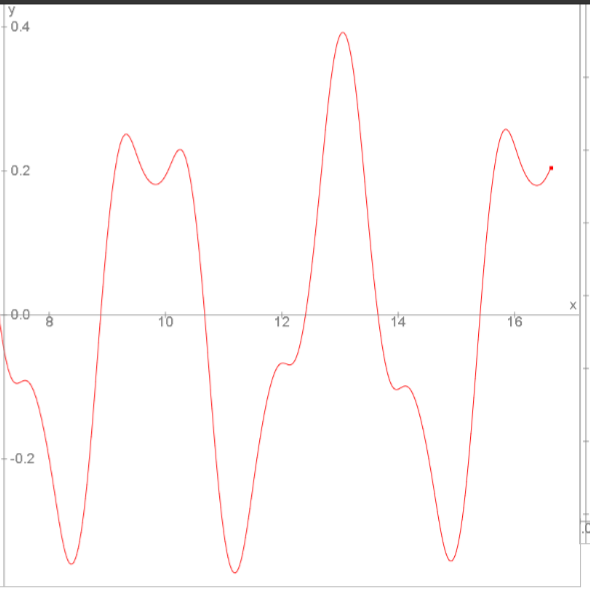
\includegraphics[width=12cm, height=8cm]{Figures/M 4b angle 1.png} % Example image
	\caption{Time series for double pendulum ($\theta_{1}$ vs t)}
\end{figure}

Below shown is the Time series for the double pendulum w.r.t m2:
\begin{figure}[h] % [h] forces the figure to be output where it is defined in the code (it suppresses floating)
	\centering
	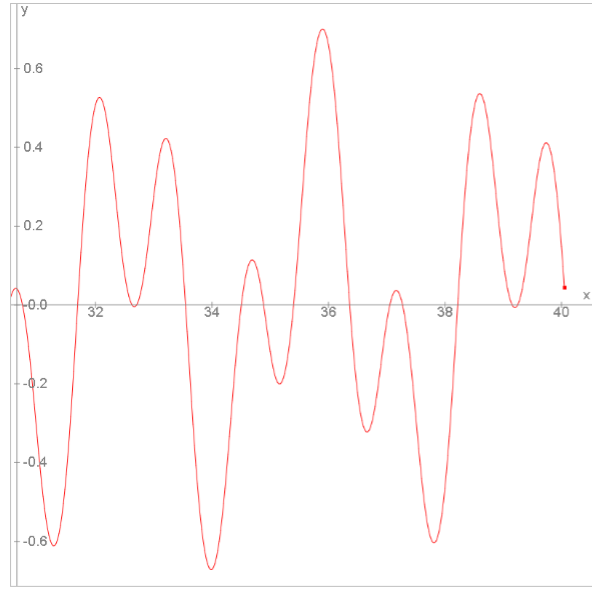
\includegraphics[width=12cm, height=8cm]{Figures/M 4b angle 2.png} % Example image
	\caption{Time series for double pendulum ($\theta_{2}$ vs t)}
\end{figure}

\newpage
\subsection{Anshul Jindal(IMT2020039)}

\textbf{1}.
Acceleration due to gravity (g) as reported by phyphox by using phone as a simple pendulum is = 9.34$m/s^2$\\

\textbf{2a}.
Phase portrait of a simple pendulum without dissipation is an ellipse.\\
Three different values of the amplitude($\theta$) taken by me is: 0.8, 0.4 and 0.2\\

The plot for phase portrait for all of them is shown below:

\begin{figure}[h] % [h] forces the figure to be output where it is defined in the code (it suppresses floating)
	\centering
	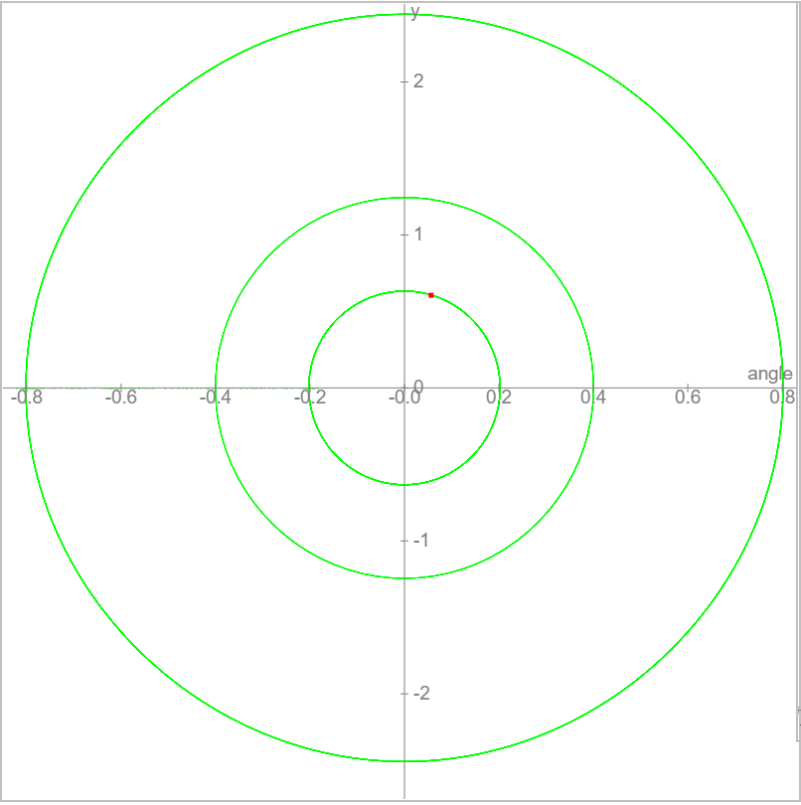
\includegraphics[width=\textwidth, height=15cm]{2a.PNG} % Example image
	\caption{Phase portrait for amplitude 0.8, 0.4 and 0.2 .}
\end{figure}

\newpage
\textbf{2b}.
Phase Portrait of the desired experiment is:
\begin{figure}[h] % [h] forces the figure to be output where it is defined in the code (it suppresses floating)
	\centering
	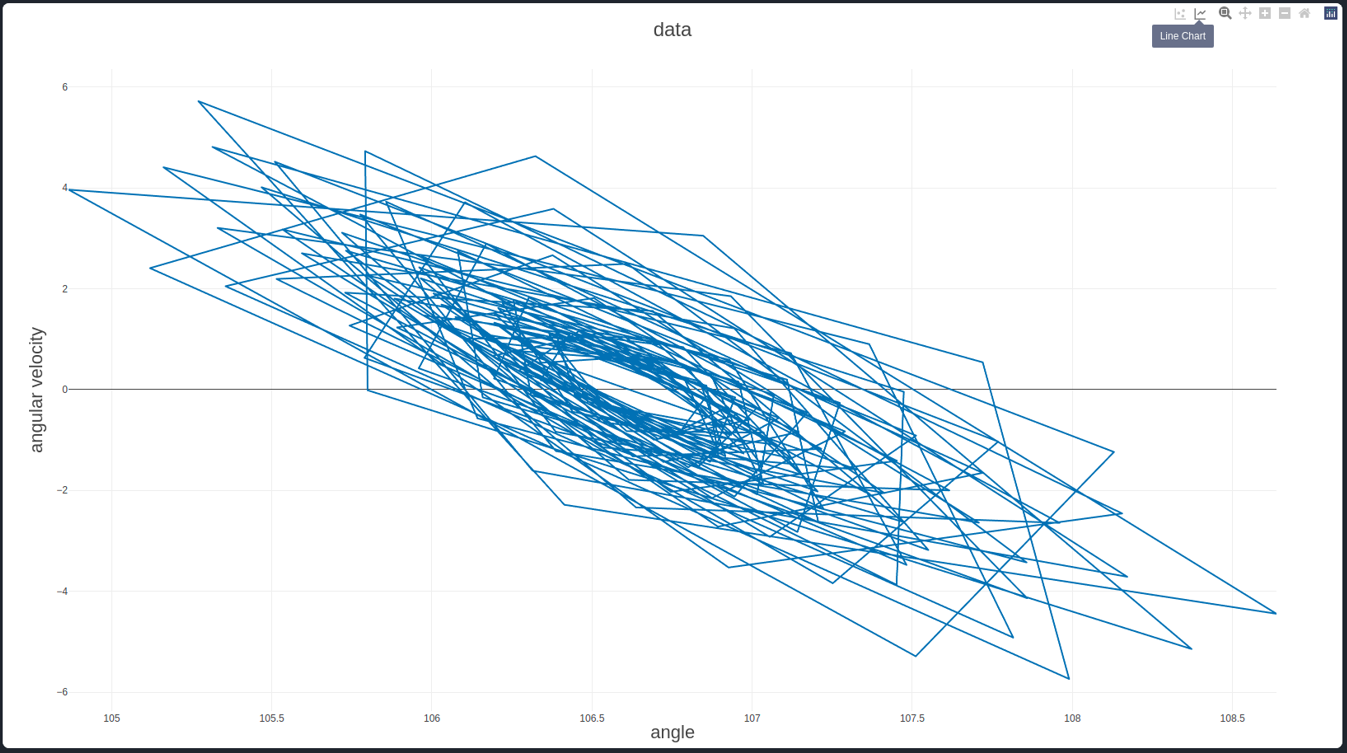
\includegraphics[width=12cm, height=8cm]{Anshul_2b.PNG} % Example image
	\caption {Representative phase portrait for your smartphone-pendulum}
\end{figure}

\textbf{2c}.
Time series of the desired experiment is:
\begin{figure}[h] % [h] forces the figure to be output where it is defined in the code (it suppresses floating)
	\centering
	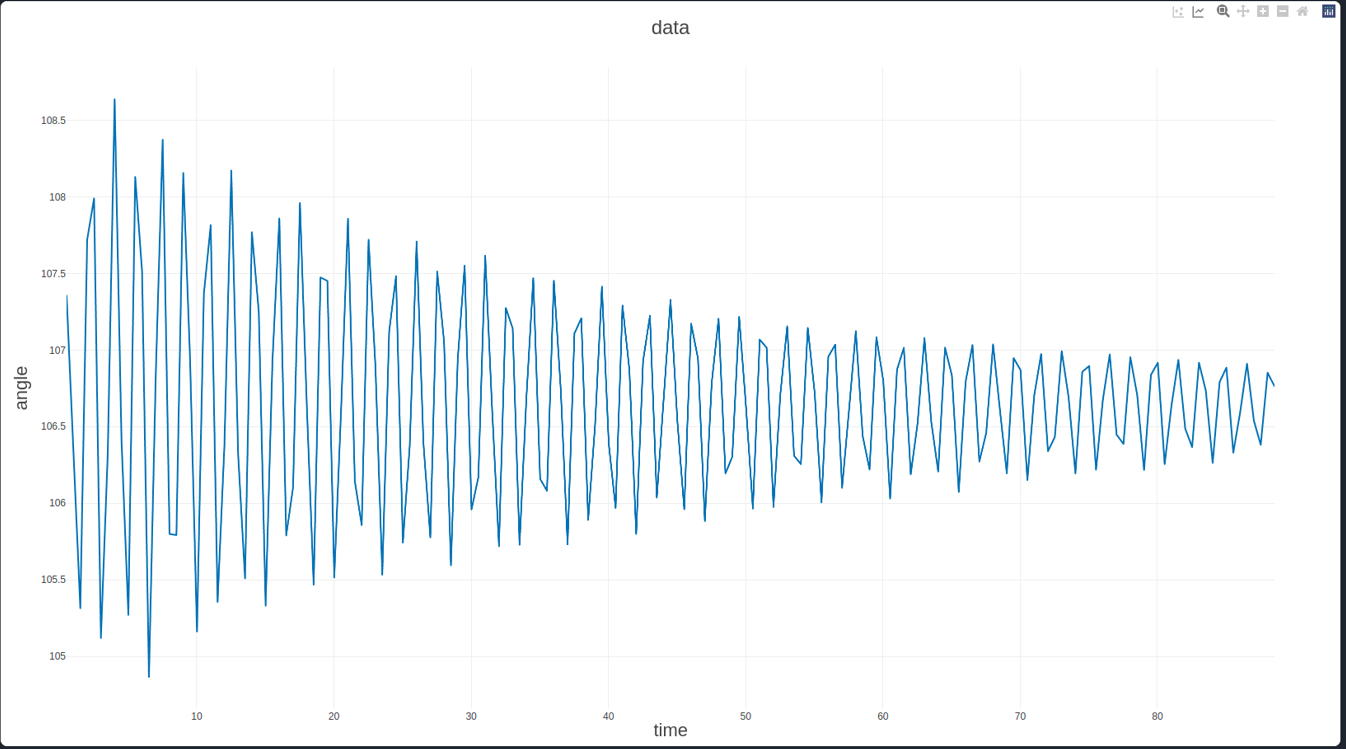
\includegraphics[width=12cm, height=8cm]{Anshul_2c.PNG} % Example image
	\caption {Representative Time series for your smartphone-pendulum ($\theta$ vs t)}
\end{figure}

\newpage
\textbf{3}.
Non-zero value for the drag chosen by me = 0.130 \\
I got concentric ellipses. Phase portrait is shown below:
\begin{figure}[h] % [h] forces the figure to be output where it is defined in the code (it suppresses floating)
	\centering
	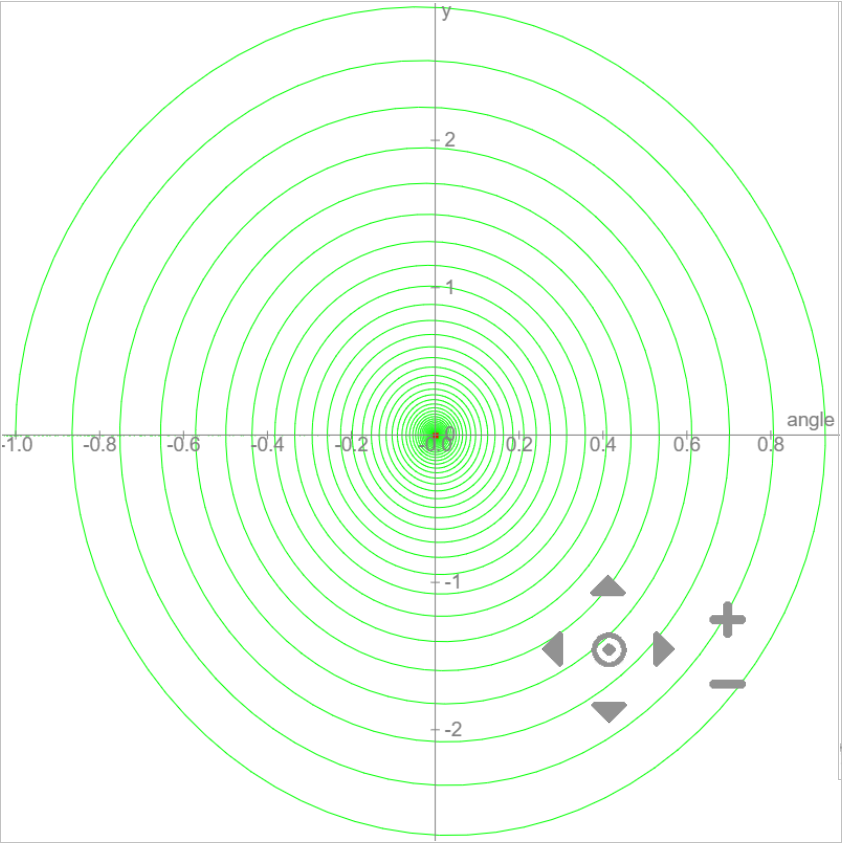
\includegraphics[width=\textwidth, height=15cm]{3.PNG} % Example image
	\caption{Phase portrait for simple pendulum in presence of drag.}
\end{figure}

\textbf{$1^{st}$ Ellipse - }\\
length of major axis (a) = 2.54 units\\
length of minor axis (b) = 0.87 units\\

So area will be (A) = $\pi$ab \implies 2.54*0.87*$\pi$ \implies 2.21$\pi$ units\\
\textbf{$2^{nd}$ Ellipse - }\\
length of major axis (a) = 2.22 units\\
length of minor axis (b) = 0.76 units\\

So area will be (A) = $\pi$ab \implies 2.22*0.76*$\pi$ \implies 1.69$\pi$ units\\

\textbf{$3^{rd}$ Ellipse - }\\
length of major axis (a) = 1.95 units\\
length of minor axis (b) = 0.66 units\\

So area will be (A) = $\pi$ab \implies 1.95*0.66*$\pi$ \implies 1.29$\pi$ units\\

\textbf{Quantifying Energy Lost:}\\
Between Ellipse 1 and Ellipse 2:\\

Area of ellipse 1 (A1) = 2.21$\pi$ units\\
Area of ellipse 2 (A2) = 1.69$\pi$ units\\

Now percentage decrease in area:
\begin{equation*}
\implies (\frac{A1-A2}{A1})*100
\end{equation*}

\begin{equation*}
\implies (\frac{2.21\pi-1.69\pi}{2.21\pi})*100
\end{equation*}

\begin{equation*}
\implies 23.53 \%
\end{equation*}

Between Ellipse 2 and Ellipse 3:\\

Area of ellipse 2 (A2) = 1.69$\pi$ units\\
Area of ellipse 3 (A3) = 1.29$\pi$ units\\

Now percentage decrease in area:
\begin{equation*}
\implies (\frac{A2-A3}{A2})*100
\end{equation*}

\begin{equation*}
\implies (\frac{1.69\pi-1.29\pi}{1.69\pi})*100
\end{equation*}

\begin{equation*}
\implies 23.66 \%
\end{equation*}

\textbf{Observation:}
The percentage decrease in area is almost equal for all the consecutive concentric ellipses.\\

\textbf{4a}.
I have taken \textbf{l1} and \textbf{l2} both equal to 0.836 units such that \textbf{L}=$\frac{l2}{l1}$ = 1 units\\

The phase portraits and time series graphs are shown in next page.

The value of \textbf{M} chosen by me is $\frac{1}{3}$ units for which I took \textbf{m1} as 2.00 units and \textbf{m2} as 1.00 units.\newpage

\textbf{Phase Portrait:}\\
Below shown is the phase portrait for the double pendulum w.r.t m1:
\begin{figure}[h] % [h] forces the figure to be output where it is defined in the code (it suppresses floating)
	\centering
	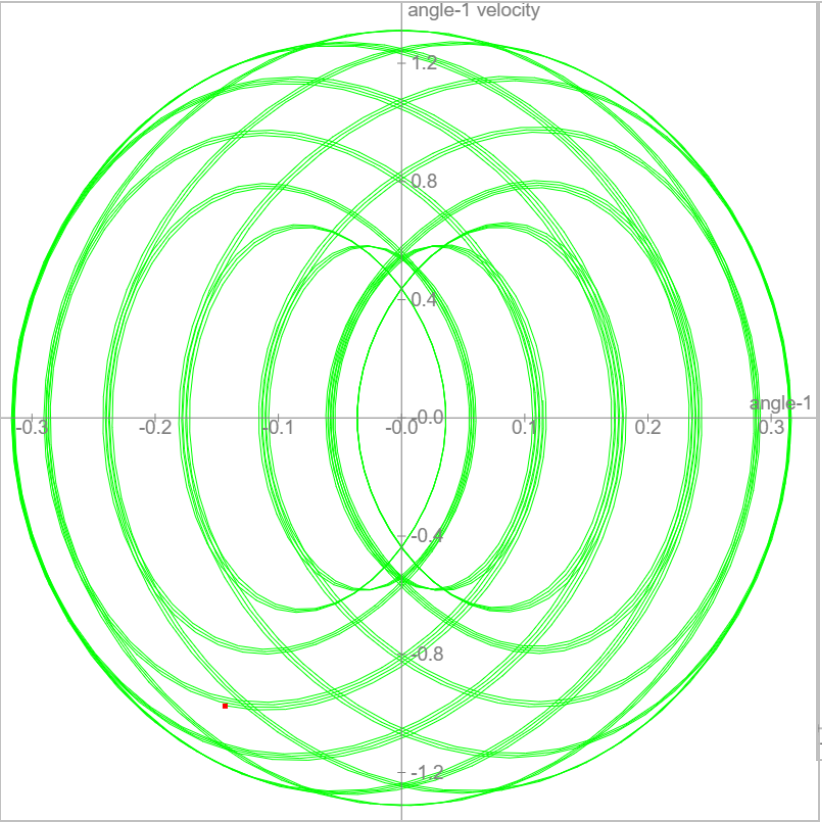
\includegraphics[width=12cm, height=8cm]{4a_phase(1).PNG} % Example image
	\caption{Phase portrait for double pendulum (d$\theta_{1}$/dt vs $\theta_{1}$)}
\end{figure}
\\
Below shown is the phase portrait for the double pendulum w.r.t m2:
\begin{figure}[h] % [h] forces the figure to be output where it is defined in the code (it suppresses floating)
	\centering
	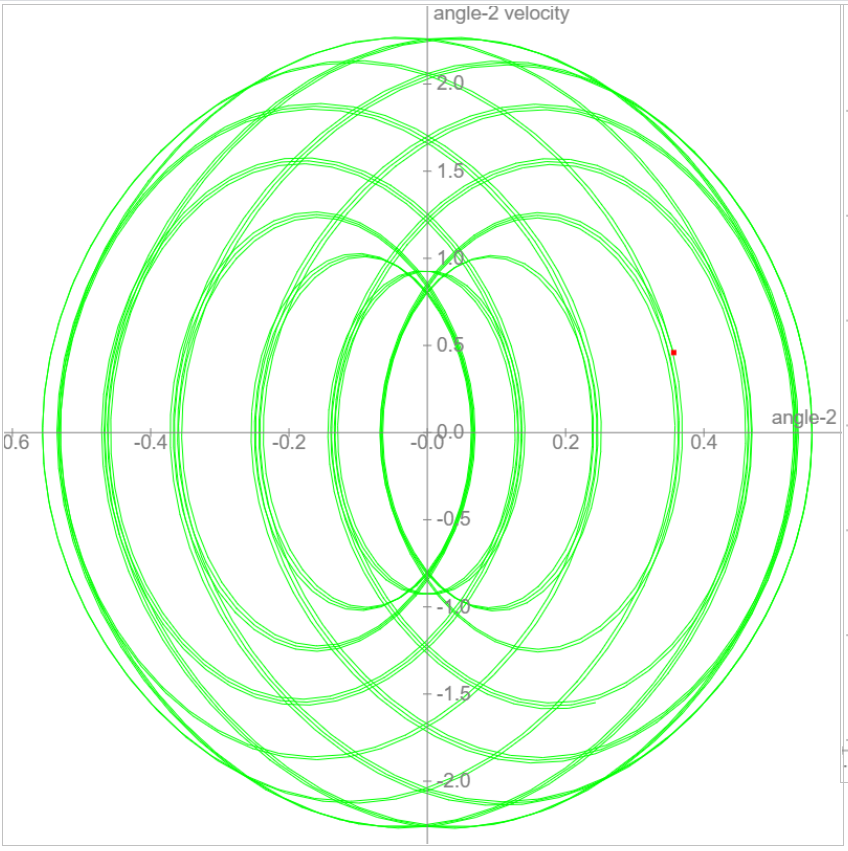
\includegraphics[width=12cm, height=8cm]{4a_phase(2).PNG} % Example image
	\caption{Phase portrait for double pendulum (d$\theta_{2}$/dt vs $\theta_{2}$)}
\end{figure}
\newpage
\textbf{Time Series:}\\
Below shown is the Time series for the double pendulum w.r.t m1:
\begin{figure}[h] % [h] forces the figure to be output where it is defined in the code (it suppresses floating)
	\centering
	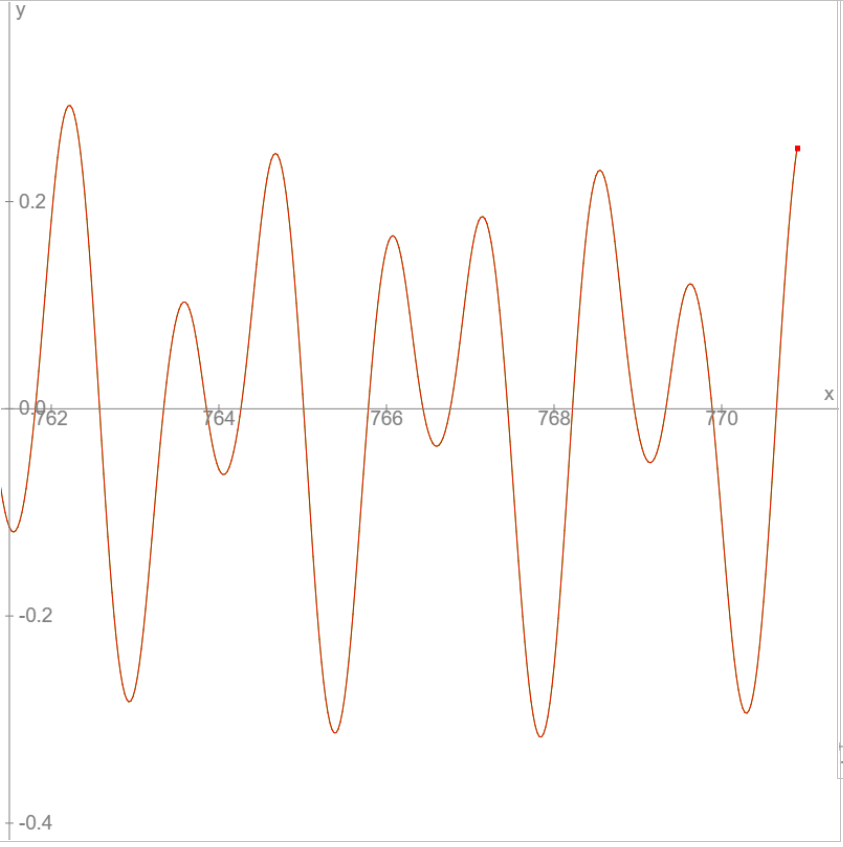
\includegraphics[width=12cm, height=8cm]{4a_time(1).PNG} % Example image
	\caption{Time series for double pendulum ($\theta_{1}$ vs t)}
\end{figure}

Below shown is the Time series for the double pendulum w.r.t m2:
\begin{figure}[h] % [h] forces the figure to be output where it is defined in the code (it suppresses floating)
	\centering
	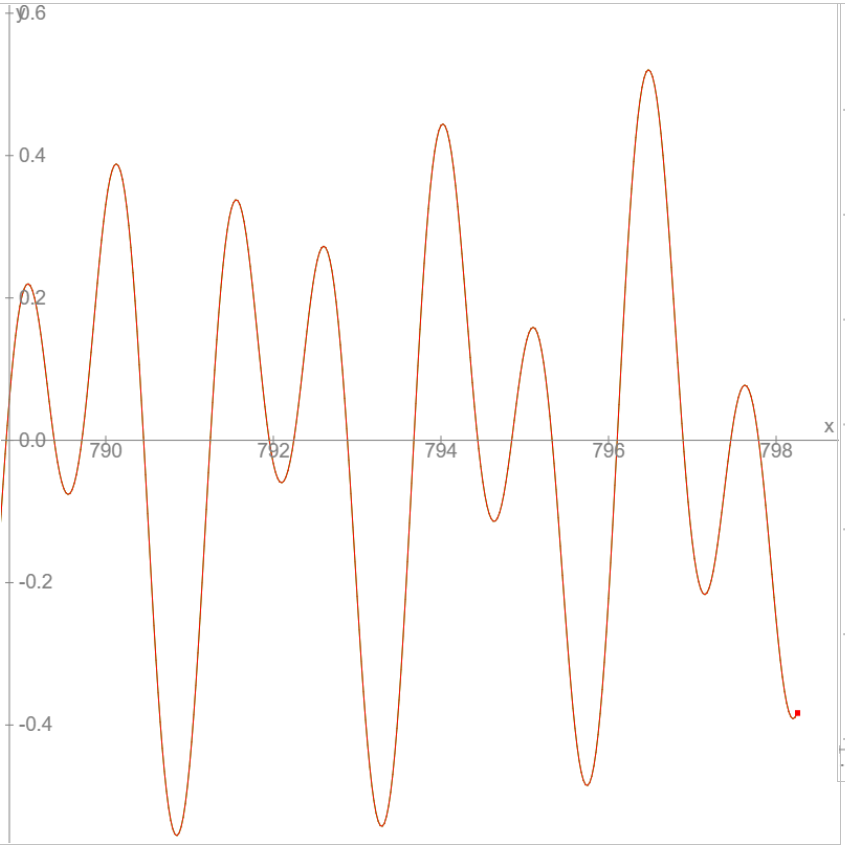
\includegraphics[width=12cm, height=8cm]{4a_time(2).PNG} % Example image
	\caption{Time series for double pendulum ($\theta_{2}$ vs t)}
\end{figure}


\newpage
\textbf{4b}.
\textbf{M} is kept constant at 0.50 units by keeping \textbf{m1} = 1.00 units and \textbf{m2} = 1.00 units as well.\\

The value of \textbf{L} chosen by me is 0.800 units by keeping \textbf{l2} = 0.800 units and \textbf{l1} = 1.000 units

\textbf{Phase Portrait:}\\
Below shown is the phase portrait for the double pendulum w.r.t m1:
\begin{figure}[h] % [h] forces the figure to be output where it is defined in the code (it suppresses floating)
	\centering
	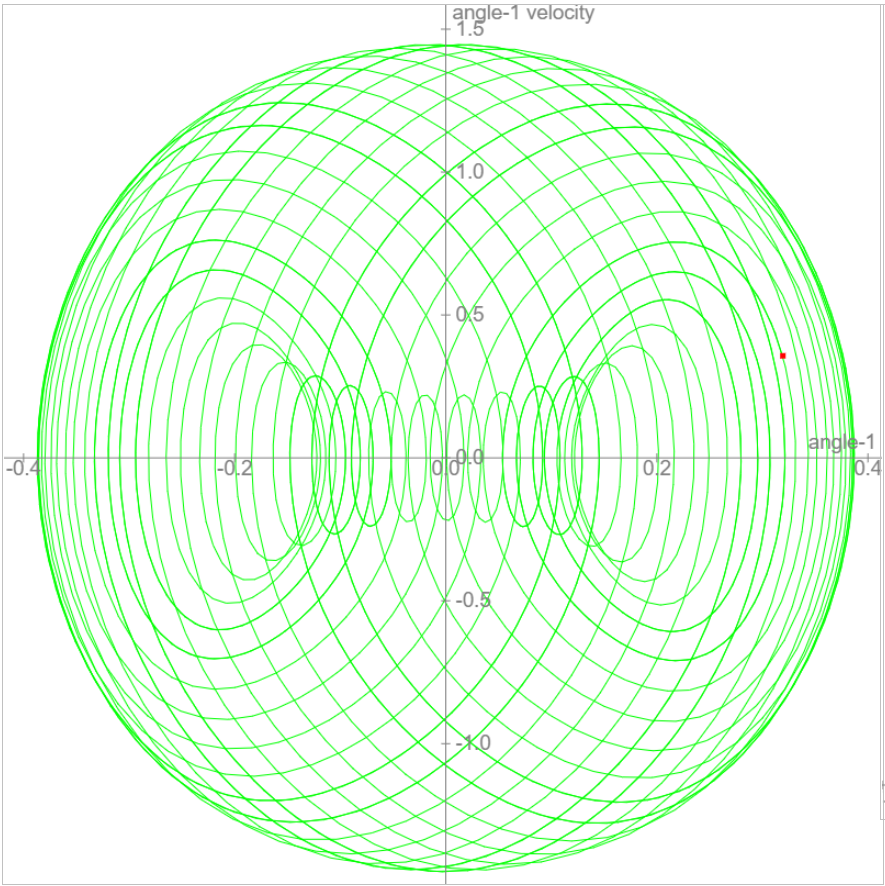
\includegraphics[width=12cm, height=8cm]{4b_phase(1).PNG} % Example image
	\caption{Phase portrait for double pendulum (d$\theta_{1}$/dt vs $\theta_{1}$)}
\end{figure}
\\
Below shown is the phase portrait for the double pendulum w.r.t m2:
\begin{figure}[h] % [h] forces the figure to be output where it is defined in the code (it suppresses floating)
	\centering
	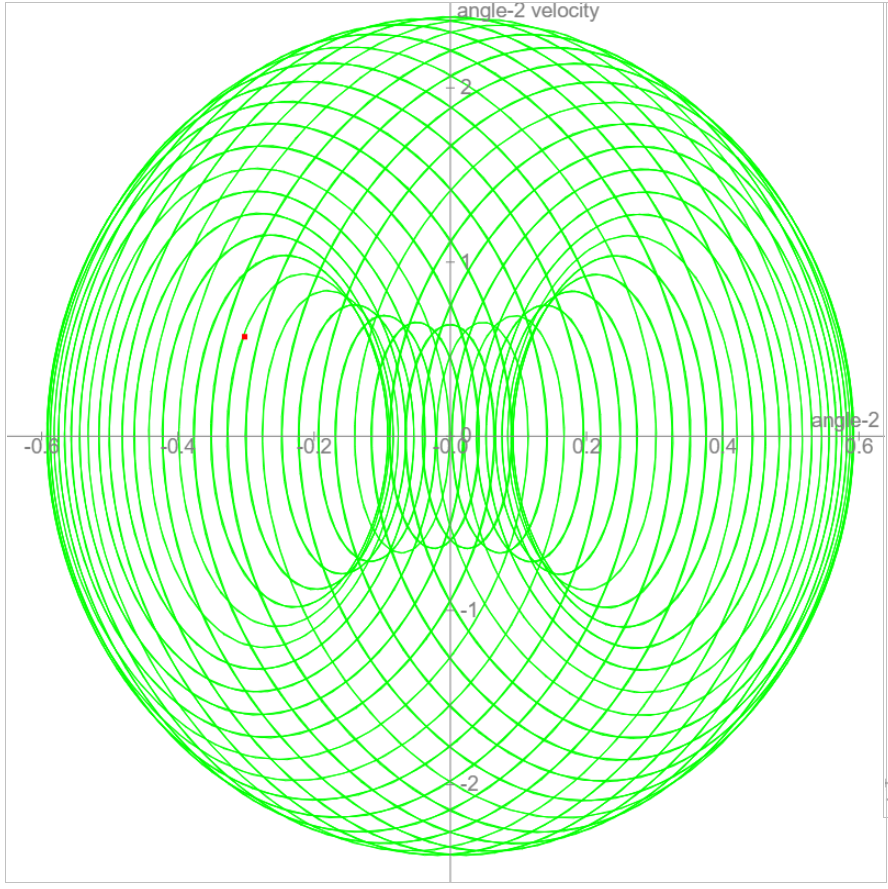
\includegraphics[width=12cm, height=8cm]{4b_phase(2).PNG} % Example image
	\caption{Phase portrait for double pendulum (d$\theta_{2}$/dt vs $\theta_{2}$)}
\end{figure}
\newpage
\textbf{Time Series:}\\
Below shown is the Time series for the double pendulum w.r.t m1:
\begin{figure}[h] % [h] forces the figure to be output where it is defined in the code (it suppresses floating)
	\centering
	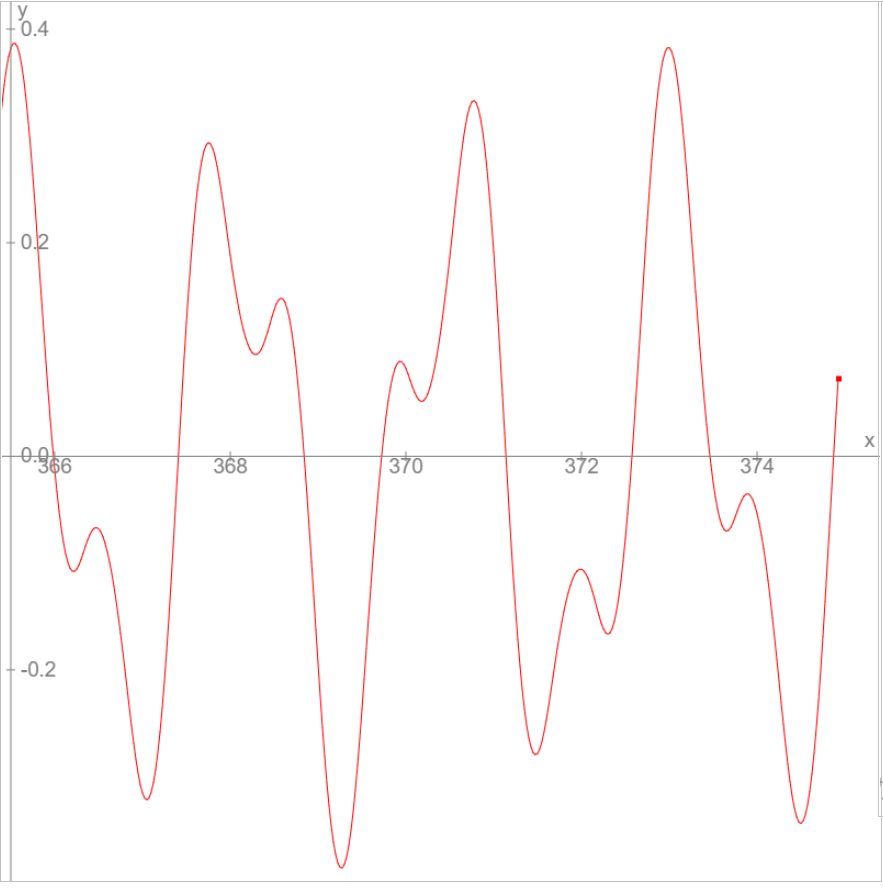
\includegraphics[width=12cm, height=8cm]{4b_time(1).PNG} % Example image
	\caption{Time series for double pendulum ($\theta_{1}$ vs t)}
\end{figure}

Below shown is the Time series for the double pendulum w.r.t m2:
\begin{figure}[h] % [h] forces the figure to be output where it is defined in the code (it suppresses floating)
	\centering
	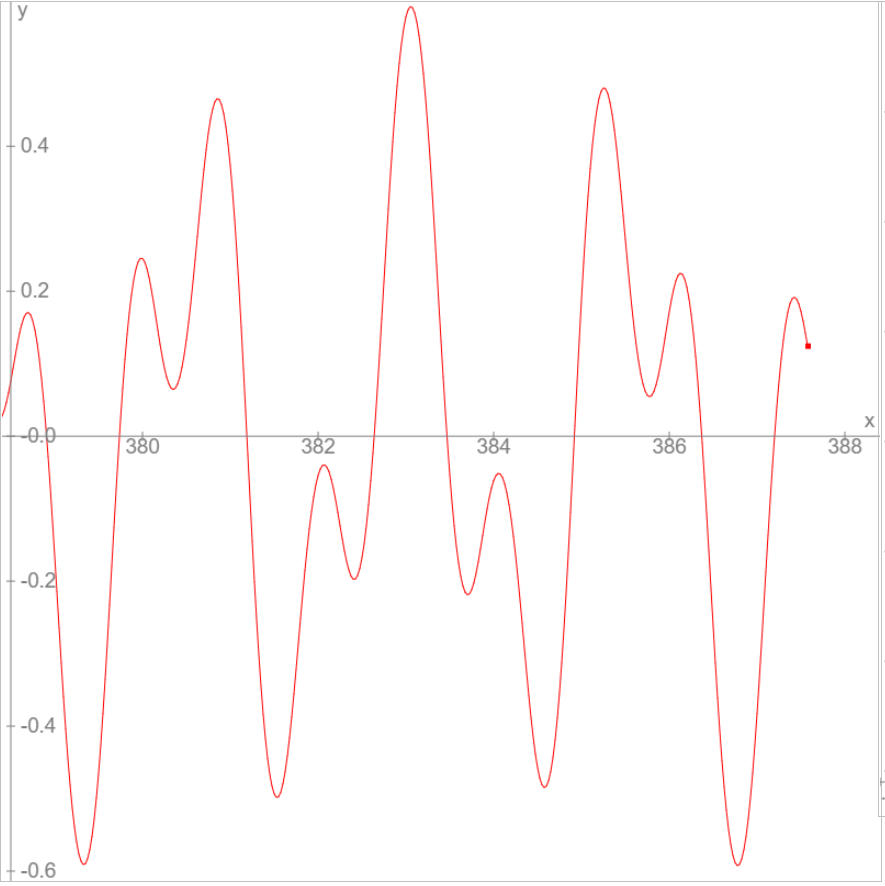
\includegraphics[width=12cm, height=8cm]{4b_time(2).PNG} % Example image
	\caption{Time series for double pendulum ($\theta_{2}$ vs t)}
\end{figure}















\end{document}